The UR20 arm is a layer controlled by the PLC used exclusively for manipulation. It is a collaborative robot arm that will be used to grab the boxes and position them upon the pallet. It has three subsystems: the movement interface, the vacuum gripper, and the vacuum gripper controller.

\begin{figure}[h!]
	\centering
 	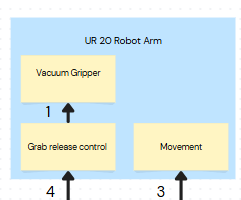
\includegraphics[width=0.60\textwidth]{images/UR20_ARM}
 \caption{UR20 Robot Arm Layer}
\end{figure}

\subsection{Movement}
This subsystem of the UR20 arm is technically an interface within the PLC, but as the PLC and UR20 are married so closely together, and this is more closely related to the arm itself, it is listed as a subsystem of the arm. The interface will allow easy control of the arm's movements. Its input is data from the PLC's decision making algorithm and its output is to directly control the robot's movements.

\subsubsection{Assumptions}
The assumption being made is that the UR20 arm is going to exclusively be a tool of the PLC, and thus will only interface with the PLC. The movement interface may even be built into the PLC for this robot, as it seems to be with some other UR cobots, but as of right now it is being assumed that a control system will have to be programmed for it on the PLC.

\subsubsection{Responsibilities}
The responsibility of the movement subsystem is to translate the box location, current arm location, and current desired speed into a coherent set of movements for the UR20 arm. These factors will be combined to create a set of movements and movement speed that will move the arm to the desired location. This must account for the position of the QR scanner when deciding where to place the arm.

\subsubsection{Movement Subsystem Interfaces}
Each of the inputs and outputs for the subsystem are defined here.

\begin {table}[H]
\caption {Movement interface} 
\begin{center}
    \begin{tabular}{ | p{1cm} | p{6cm} | p{3cm} | p{3cm} |}
    \hline
    ID & Description & Inputs & Outputs \\ \hline
    \#08 & Change in X,Y,Z Coordinates & \pbox{3cm}{X \\ Y \\ Z} & \pbox{3cm}{NO OUTPUT}  \\ \hline
    \#09 & Movement Speed & \pbox{3cm}{Speed} & \pbox{3cm}{NO OUTPUT}  \\ \hline
    \#10 & Rotation Angles & \pbox{3cm}{Perpendicular \\ Longitudinal} & \pbox{3cm}{NO OUTPUT}  \\ \hline
    \end{tabular}
\end{center}
\end{table}

\subsection{Vacuum Gripper}
    The vacuum gripper is physical hardware and its software inputs and outputs are covered in the Vacuum Gripper Controller subsystem. The vacuum gripper is connected to a vacuum generator that will be adjusted to provide a static amount of force capable of picking the boxes and not dropping them until the controller determines that it should do so.

\subsubsection{Assumptions}
The vacuum gripper will be a hardware-only system with a constant vacuum that can be blocked in order to drop a box. It will interface exclusively with the vacuum gripper controller and have no outputs.

\subsubsection{Responsibilities}
The responsibility of the vacuum gripper is to securely hold and transport boxes. It will be able to drop the boxes on command and in the process it will shift the boxes as little as possible in order to produce the expected placement.

\subsubsection{Movement Subsystem Interfaces}
Each of the inputs and outputs for the subsystem are defined here.

\begin {table}[H]
\caption {Movement interface} 
\begin{center}
    \begin{tabular}{ | p{1cm} | p{6cm} | p{3cm} | p{3cm} |}
    \hline
    ID & Description & Inputs & Outputs \\ \hline
    \#11 & Vacuum Control Signal & \pbox{3cm}{ONOFF} & \pbox{3cm}{NO OUTPUT}  \\ \hline
    \end{tabular}
\end{center}
\end{table}

\subsection{Vacuum Gripper Controller}
The vacuum gripper controller is the software interface between the PLC and the vacuum gripper. It signals the vacuum hardware to kill the vacuum and drop the box being held. 

\subsubsection{Assumptions}
The vacuum gripper controller will be on at all times EXCEPT when it is told that a box needs to be dropped. 

\subsubsection{Responsibilities}
The vacuum gripper controller must turn off the vacuum long enough for the cobot to move away, which should occur soon after. If it turns on again too soon, the box will be pulled out of the desired position. 

\subsubsection{Movement Subsystem Interfaces}
Each of the inputs and outputs for the subsystem are defined here.

\begin {table}[H]
\caption {Movement interface} 
\begin{center}
    \begin{tabular}{ | p{1cm} | p{6cm} | p{3cm} | p{3cm} |}
    \hline
    ID & Description & Inputs & Outputs \\ \hline
    \#12 & Drop Signal & \pbox{3cm}{Trigger} & \pbox{3cm}{ONOFF}  \\ \hline
    \#13 & Current Speed & \pbox{3cm}{Speed} & \pbox{3cm}{NO OUTPUT}  \\ \hline
    \end{tabular}
\end{center}
\end{table}

